\chapter{Measuring the plasma expansion}\label{ch:Measuring the gradient expansion}
\minitoc
\thispagestyle{empty}
\section{Spatial Domain Interferometry (SDI)}

\subsection{Introduction}

When the intensity of a pulse interacting with matter exceeds $\sim 10^{11}\,\mathrm{W/cm^2}$, ionization takes place and any solid material turns into a plasma. 
The zero pressure inside the experimental chamber does not balance the plasma thermal pressure (typically $T\sim 100\,\mathrm{eV}$ ) which consequently expands towards vacuum at approximatively the speed of sound ($c_s\sim 10\,\mathrm{nm/ps}$). 
 The characteristic spatial and temporal expansion scale lengths ($<10\,\mathrm{nm}$, $<1\,\mathrm{ps}$ respectively) make femtosecond (fs) laser pulses the best candidates to perform accurate measurements using phase-sensitive detection schemes such as Frequency Domain Interferometry (FDI)~\cite{Geindre1994,evans1996time,quoix2000ultrafast,audebert2001direct,geindre2001single}. The principle of FDI is as follows:\\
A probe beam of short duration (several fs) is split into two copropagating replicas separated by an adjustable delay. The first replica is reflected by the target in the absence of plasma, and the second is reflected after the plasma expansion has been triggered by a pump pulse. Both replicas are sent into an imaging spectrometer to visualize the spectral modulations resulting from their interference. In the region of space where the second replica was phase shifted because of plasma expansion, the changes in the spectral pattern enable the reconstruction of the plasma spatial profile for a given pump-probe delay.
 
 Although FDI can reach $\lambda /2000$ resolution~\cite{Geindre1994}, it is rather complex to implement on a running plasma mirror experiment. In this chapter, we present a technique we developed called Spatial Domain Interferometry (SDI). It is easier to implement experimentally, based on time-resolved spatial phase-shift imaging interferometry. We present the basic principle of the technique and show experimental results applied to the characterization of the gradient generated by our controlled prepulse.\\
 
  % Our experimental setup was already described in section~\ref{section:Solid target experimental set-up}. Here, we by pass the telescope from the compression chamber.\\


\subsection{Basic principle} \label{subsubsection:Principle of the method}

We showed in the previous section that the main pulse was used to generate high-order harmonics on a solid target after it is ionized by prepulse with adjustable delay. For a SDI measurement of the plasma expansion, we transform the "main pulse" into a "plasma expansion probe pulse" by adding a periodic transmission mask in the main beam path prior to the focusing parabola. The mask is a simple blocker with periodic holes represented in Fig~\ref{fig:ScemePrinciple_SDI}(a), which causes a diffraction pattern in the focusing plane where we can identify several diffraction orders as represented in Fig~\ref{fig:ScemePrinciple_SDI}(b).
The spacing between the $0^{th}$ order and the first-order ring is chosen such that only the $0^{th}$ order is reflected by the expanded plasma, represented with orange color in Fig~\ref{fig:ScemePrinciple_SDI}(b). In this configuration, only one order is phase shifted as the probe is reflected by the plasma, the other orders impinge on a non-irradiated target surface. This ultimately leads to intensity modulations of the far-field after propagation as illustrated in Fig~\ref{fig:ScemePrinciple_SDI}(c) for a phase shift of respectively $\Delta \phi =0$ and $\pi$. The principle of SDI is therefore to retrieve the shape of the plasma and its expansion velocity from these spatial intensity modulations.\\

%The reflection of the central diffraction spot by the peak of the plasma mirror surface induces a phase shift relative to the higher order diffraction spots around it, leading in turn to a clearly observable time-dependent spatial interference pattern in the far-field intensity profile of the reflected probe beam.



\begin{figure}[H]
\centering
\includegraphics[width =1\textwidth]{../chapitre7/images/ScemePrinciple_SDI.pdf}\\
\caption{\label{fig:ScemePrinciple_SDI} SDI principle applied to ultrafast plasma mirror imaging: the probe field $E(x,y)$ is diffracted by a transmission mask $T_M$(a) onto a plasma mirror in the focusing plane (b). The phase shift, $\Delta\phi$, of the central diffraction spot induced by the plasma expansion leads to a modulation of the far-field spatial intensity profile(c) of the reflected probe with respect to $\Delta\phi$.}
\end{figure}


\noindent We designate by $T_M$ the transmission mask introduced in the collimated probe beam prior to the focusing optic of focal length $f$. As a consequence, the probe pulse focus spot splits into several spots spaced by $\Delta x =
\frac{\lambda f}{a}$, where $a$ is the period of the mask and $\lambda$ the central wavelength. The probe field after the mask is defined by:

\begin{align} E_M(x,y,\omega) = E(x,y,\omega)T_M(x,y).\end{align}

\noindent Within the paraxial approximation, the field $E_{ref}$ in the focusing is given by:

\begin{align} E_{ref}(x,y) = \mathscr{F}[E_M](\nu_x = \frac{x}{\lambda f},\nu_y = \frac{y}{\lambda f})\end{align}

\noindent where $\mathscr{F}$ denotes the spatial Fourier transform, and ($\nu_x$,$\nu_y$) the spatial frequencies.
As shown in Fig~\ref{fig:ScemePrinciple_SDI}, the expanding reflective plasma introduces a phase shift where it spatially overlaps with $E_{ref}$. We designate its effect on the reference field 
by the complex transfer function $T$ which allows us to define a new field:

\begin{align} \label{eq:OnFocus} E_2(x,y) = E_{ref}(x,y)T(x,y)
\end{align}

\noindent where $T= |T|e^{i\phi}$ is the transfer function of the plasma. $|T|\ne 1$ is therefore equivalent to a variation of the reflectivity.

\noindent We finally call $E_F$ the field after propagation and far from the plasma surface ($z>>Z_R$) which can be calculated by Fourier transform of Eq~\ref{eq:OnFocus}:

\begin{align} \label{eq:FarField} E_{F}(x,y) = \mathscr{F}[E_2](\nu_x = \frac{x}{\lambda f},\nu_y = \frac{y}{\lambda f}).\end{align}

\noindent We recall the property of the Fourier transform of a function $f$:
$$(\mathscr{F}^{-1} f) (x) = (\mathscr{F}.f)(-x)
$$
\noindent This ultimately implies the identity $\mathscr{F}[\mathscr{F}.f](x) = f(-x)$ and we can write:

\begin{subequations}
\label{equation-motion-pond2}
\begin{align}[left = \empheqlbrace\,]
&\label{eq:FarField2} E_{F}(x,y) = \mathscr{F}\Bigl(\mathscr{F}[E_M] T \Bigr)(\nu_x = \frac{x}{\lambda f},\nu_y = \frac{y}{\lambda f})\\
&\label{eq:FarField3}  E_{F}(x,y) = E_M(-x,-y) + \mathscr{F}\Bigl(\mathscr{F}[E_M](T-1)) 
\end{align}
\end{subequations}



\noindent Using the relation $\mathscr{F}(fg) = \mathscr{F}(f)*\mathscr{F}(g)$, we can verify that the reflected intensity $I = |E_{F}|^2$ is equal to (we replace $(-x,-y)$ by $(x,y)$ in Eq~\ref{eq:FarField3} for better clarity):

\begin{align} \label{eq:Intensity} I(x,y) = |ET_M + \iint ET_M(x-x',y-y')h(x',y')dx'dy'|^2, \end{align}

\noindent where

\begin{align} h(x,y) = FT(T-1)(\frac{x}{\lambda f},\frac{y}{\lambda f}).\end{align}

\noindent The information about the plasma response is therefore contained in the function $h$. When $T=1$, we find the trivial result that $I = |ET_M|$, which means that the plasma behaves as a perfect mirror. 

\subsection{Illustration with a step-like density profile}


\noindent To estimate the effect of the plasma mirror-induced phase shift on the reflected image, we can make the simple assumption that all diffracted spots are reflected equally by the plasma and that only the $0^{th}$-order is phase shifted by a spatially uniform $\phi_0$. Mathematically, this translates into $|T| = 1$ and $\phi(x,y) = \phi_0$ for $|x|,|y| < \frac{\lambda f}{2a}$. This allows us to express $h$ by limiting the Fourier integration domain to $[-\frac{\lambda f}{2a} \  \frac{\lambda f}{2a}]$, such that:

\begin{align} h(x,y) = (e^{i\phi_0}-1)\left(\frac{\lambda f}{a}\right)^2{\rm sinc}(\frac{x}{2a}){\rm sinc}(\frac{y}{2 a}) \label{eq:f}.\end{align}

\noindent This particular solution shows that the convolution function, $h$, is periodic with $\phi_0$ since the interference term in Eq~\ref{eq:Intensity} leads to an inversion of the far-field pattern every time $\phi_0 = \pi [\pi]$. It is this periodicity that confers SDI the ability to directly visualize the monotonic expansion of the plasma mirror surface.\\

\noindent Our experiment is however different from this ideal case because the plasma mirror spatial shape is inherited from the prepulse spatial profile which differs from the step like case, and is closer to a Gaussian profile. This, however, does not prevent the inversions from being visible in the far-field intensity pattern, as we will see in the following section.




%\section{Plasma expansion measurement using simple model}


\subsection{Plasma expansion model}\label{subsubsection:Plasma exansion model}

 The description of the plasma along the target normal has already been done in subsection~\ref{subsubsection:Collective response of density gradient} and we saw it was described by a decreasing exponential of gradient scale length $L$. The plasma expansion in vacuum is a standard problem solved by Kruer~\cite{kruer1988physics} using the isothermal equation of state for the electrons  and its solution is given by the self-similar solution:

\begin{align}
n_e(x,t) = n_{c}\mathrm{exp}(-\frac{x-x_c(t)}{c_s t})
\label{eq:one}.
\end{align}

\noindent where $c_s= (Zk_bT_e/m_i)^{1/2}$ is the ion sound velocity and $n_c = (\omega_0^2m_e\epsilon_0)/e^2$  the critical density. In these expressions, $Z$ is the ion charge state, $e$ is the electron elementary charge, $k_b$ the Helmholtz constant, $T_e$ the electron temperature, $m_e$ and $m_i$ respectively the electron and ion mass. 

\begin{figure}[H]
\centering
\includegraphics[width =0.8\textwidth]{../chapitre7/images/GradientExpansion.pdf}\\
\caption{\label{fig:GradientExpansion}Illustration of gradient expansion with $c_s = 10\,\mathrm{nm/ps}$ for a prepulse delay of respectively $t = 0,2$ and $10$ps. The initial gradient scale length is taken $\delta L = \lambda / 100$. The IR probe pulse is shown to reflect 
on the critical density at respectively 2 and 10ps.}
\end{figure}



\noindent In~\ref{eq:one} we clearly identify $L(t) = c_s t$ as the gradient length which is proportional to $x_c(t)$, the coordinate of the critical density where the probe is reflected, as represented in Fig~\ref{fig:GradientExpansion}. For a fully ionized silica target the overdense maximum density is about $250n_c$ such that $x_c(t) = \ln(250)L(t) \approx 5.5 L(t)$. 

\noindent Assuming the electron temperature $T_e$ depends linearly on the energy deposited on target when the plasma is created, that is to say on the prepulse intensity $I_p$, we can write, according to its definition, that for a fixed pulse duration:
$$c_s \propto \sqrt{I_p}
$$
\noindent The prepulse intensity is taken homogeneous on each isolated diffracted spot of the main pulse in order to define a corresponding expansion velocity. $I_{p,1}$ is the prepulse intensity at the center, $I_{p,2}$ on the first order diffracted spots.
\begin{equation}
\label{eq:Csirelations}
  \left\{
      \begin{aligned}
     &c_{s,1} \propto \sqrt{I_{p,1}}\\
     &c_{s,2} \propto \sqrt{I_{p,2}}\\
      \end{aligned}
    \right.
\end{equation}

\noindent This means that the center of the plasma expands faster than its edges for a Gaussian shaped prepulse. \\

\noindent \g{Phase shift due to the expansion:}\\
Taking into account the angle of incidence of $\theta$ with respect to the target normal, we express the phase difference $\Delta\phi$  between the zero and first-order probe spots as a function of the relative critical surface position difference $\Delta x_c(t) = x_{c,1}(t) - x_{c,2}(t)$:

\begin{align}
\Delta \phi (t) = \frac{4\pi}{\lambda}\Delta x_c(t)/\cos(\theta) 
\label{eq:phase}.
\end{align}


\noindent where the expansion velocity at the center of the prepulse ($I_p = I_{p,1}$) verifies: 
\begin{align}
\Delta x_c(t) =  \ln(n_{max}/n_c)c_{s,1}(1 - \frac{c_{s,2}}{c_{s,1}})t
\label{eq:deltaXc}
\end{align}

\noindent Using Eq~\ref{eq:phase} and Eq~\ref{eq:deltaXc} , we evaluate the expansion velocity over the $0^{th}$ order of the probe $c_s = c_{s,1}$:

\begin{align}
[c_s t] = [\ln(n_{max}/n_c)(1 - \sqrt{\frac{I_{p,2}}{I_{p,1}}})\frac{4\pi}{\lambda}/\cos(\theta)]^{-1}\Delta \phi (t)
\label{eq:Csretrieval}
\end{align}

\noindent Note that in the above derivation, we have neglected the phase shift induced by the propagation in the underdense portion of the plasma. Indeed, its contribution for a given value of $L$ can be calculated for the carrier frequency $\omega_0$:
\begin{equation}
 \phi_{u} = \frac{2\pi}{\lambda}\int_{-\infty}^{n_c}\frac{\omega_P^2(x)}{\omega_0^2}dx = 4\pi\frac{L}{\lambda}
\end{equation}

Which would given rise to an additional phase difference at any time $t$:

\begin{equation}
\Delta \phi_{u}(t) = = 4\pi\frac{\Delta x_c}{5.5 \lambda}
\end{equation}

\noindent Calculating the exact phase difference for a short femtosecond pulse becomes more complex since shearing and group delays all have to be accounted for. Therefore, we neglect this term  in the following ($\Delta \phi_u /\Delta \phi \sim 0.1$) and focus on the basic principles of the exposed method. 


\subsection{Experimental setup}

The experimental pump-probe setup has already been described in Section~\ref{section:Solid target experimental set-up}.
 The  main pulse is sent through a periodically holed hexagonal mask of period $a = 4\,\mathrm{mm}$. The resulting diffraction pattern is shown in Fig \ref{fig:experimentalSetUp} were we superimposed the measured pump (gray scale) used for plasma generation and the diffracted probe (color scale) beam profiles. The central diffracted probe spot intensity is $\sim 10^{16}\,\mathrm{W/cm}^2$. The peak intensity of the prepulse is $I_{p,1} = 3.5\times 10^{14}\,\mathrm{W/cm}^2$ in the center and $I_{p,2} = 8.7\times 10^{13}\,\mathrm{W/cm}^2$ where it overlaps with the first order diffraction spots.

\begin{figure}[H]
\centering
\includegraphics[width =0.9\textwidth]{../chapitre7/images/experimentalSetUp.pdf}\\
\caption{\label{fig:experimentalSetUp} (a) Entrance slit for XUV generation (b) Silver mirror for prepulse (c) Holed mirror for main pulse (probe) (d) Transmission mask (e) Off-axis f/1.2 focusing parabola (f) Camera placed under vacum imaging the entrance slit.}
\end{figure}

\noindent Our experiment consists in recording the intensity pattern of the main pulse reflected in the specular direction as a function of pump-probe delay. No particular plane of the reflected beam is imaged, but a camera records the reflected probe beam integrated over 100 shots by imaging the anodized vertical slit usually used to block the laser before the XUV spectrometer. The results for four different pump-probe delays are displayed in the top row of Fig \ref{fig:SDIexperimentVSsimulation}. We take the intensity profile recorded at zero pump-probe delay as our reference. The first inversion of the intensity profile appears at $\simeq 12\,\mathrm{ps}$ and the second inversion occurs at
$\simeq 20\,\mathrm{ps}$. The profile inversion patterns are well reproduced by the simulations shown on the bottom row of Fig \ref{fig:SDIexperimentVSsimulation}, where we used the actual experimental pump pulse profile to simulate the phase shift due to the plasma expansion, using the model presented in subsection~\ref{subsubsection:Plasma exansion model}.


\subsection{Experimental results}

\begin{figure}[H]
\centering
\includegraphics[width =0.8\textwidth]{../chapitre7/images/SDIexperimentVSsimulation.pdf}\\
\caption{\label{fig:SDIexperimentVSsimulation} Simulated and experimental far-field probe beam intensity profile inversions at respectively $0\,\mathrm{ps}$(a) $6\,\mathrm{ps}$(b), $12\,\mathrm{ps}$(c) and $20\,\mathrm{ps}$(d) pump-probe delay. The simulations are performed using the measured pump beam profile and assuming the plasma expansion velocity $c_s\propto \sqrt{I_p}$.}
\end{figure}

\begin{figure}[H]
\centering
\includegraphics[width =0.8\textwidth]{../chapitre7/images/Cs_retrieval-error.pdf}\\
\caption{\label{fig: Cs_retrieval-error}Measurement of plasma relative expansion for a prepulse intensity of $I_{p,1} = 3.5\times 10^{14}\,\mathrm{W/cm}^2$ as a function of pump-probe delay. Each experimental point corresponds to a $\pi$ inversion in the intensity profile of the reflected probe. The corresponding linear fit allows one to retrieve a plasma expansion velocity of $c_s\approx 10.8\,\mathrm{nm/ps}$}
\end{figure}

\noindent The phase inversion corresponding to the experimental data points reported in Fig~\ref{fig: Cs_retrieval-error} are identifiable by eye, and the corresponding error bar increases with pump-probe delay (inversion become less and less clear because energy fluctuations of the pump pulse impact the expansion velocity of the plasma).\\
A few important remarks need to be made about that measurement technique so far:\\

\begin{itemize}
\item[$\bullet$] The retrieved $c_s$ is intrinsically contingent on the hypothesis that the expansion velocity in vacuum is proportional to the square root of the pump laser intensity. An absolute measurement of the expansion would require phase retrieval for any pump-probe delay rather than looking for inversions supposedly corresponding to $\Delta\phi = n\pi$ where $n$ is integer. This point will be developed in Section~\ref{section:Phase retrieval perspective}. In addition, note that we measure the expansion of the critical surface. The proportionality factor between this surface and the gradient length $L$ is based on the hypotheses that the plasma has an exponential profile and that the electron temperature does not vary during the expansion. Any violation of these hypotheses leads to an error on the retrieved gradient length $L$.

\item[$\bullet$] The error bars in Fig~\ref{fig: Cs_retrieval-error} do not take into account the fact that the relative position between the pump and probe beam (and consequently the relative intensity $I_{p,1}$ and $I_{p,2}$) changes during an experiment. The pointing stability can degrade over several hours, or thermal lens effects in the chain can lead to both beam going out of alignment when they are attenuated as we describe in~\ref{subsubsection:Break of symetry}. This could ultimately lead to an error bar of the order the $c_s$ which is why the previous measurement should only be considered as a proof-of-principle at this time. 

\item[$\bullet$] Similar to the fs pump-probe spatial imaging technique employed in \cite{Downer1985}, our time resolution is simply limited by the duration of the pulse used to probe the plasma expansion induced by the pump pulse.

\end{itemize}

\vspace{0.1in}

\noindent As a conclusion, we have demonstrated the basic proof-of-principle of SDI but a lot of effort needs to be made to improve the beam stability at full power to properly evaluate the error bar relative to the measurement as illustrated in the following section.

\section{Sensitivity to beam alignment}

\subsection{Single-order phase shift and experimental limitations}

In the previous experiment, we were in a configuration where the first diffracted orders where also affected by the plasma expansion because the diffraction spacing~$r$ was not large enough.

\begin{figure}[H]
\centering
\includegraphics[width =0.7\textwidth]{../chapitre7/images/Principle.pdf}\\\caption{\label{fig:Principle} Definition of the variables $a$: mask spacing, $T$: plasma transfer function on target, $E_{ref}$: field on target when $T=1$, $E_{ref,0}$: $0^{th}$ order diffracted spot on target, $E_{exp}$: field on target for arbitrary $T$, $r$: distance from center to first diffraction order, $\Sigma$: reflected far-field conjugate to mask holes, $\bar{\Sigma}$: reflected far-field conjugate to mask}
\end{figure}

\noindent If we suppose that for a laser intensity $I_p < I_{lim} = 10^{10}\,\mathrm{W/cm^2}$ , neither ionization nor small phase distortions of the surface affect the reference field $E_{ref}$, we find a \g{separation spacing criterion} for the diffracted spot for a prepulse intensity~$I_p$ :

\begin{equation}
r > (d_{1/2}/2)\sqrt{\ln(I_p/I_{lim})/\ln(2)}
\end{equation}

\noindent Where $r$ is the distance from the center to the first diffracted spot  represented in Fig~\ref{fig:Principle}, and $d_{1/2}$ the prepulse spatial FWHM.
Using this constraint, we can retrieve a maximum period for the transmission mask:

\begin{equation}
a= \frac{\lambda f}{r} < \frac{\lambda f}{d_{1/2}/2\sqrt{\ln(I_p/I_{lim})/\ln(2)}}
\end{equation}

\noindent In our experimental conditions where $5\times 10^{14}\,\mathrm{W/cm^2}$, $d_{1/2} \approx 22\,\mathrm{\mu m}$, this implies that $ r \gtrsim 2 d_{1/2}$ which for $\lambda = 800\,\mathrm{nm}$ gives:
$$
a \lesssim 960 \,\mathrm{\mu m}
$$

\noindent We designed masks with spacing matching this separation condition by drilling holes in metal banks using the smallest available drill diameter ($\sim 0.8\mathrm{mm}$). 

\begin{figure}[H]
\centering
\includegraphics[width =\textwidth]{../chapitre7/images/DifferentMasksComparaison.pdf}\\
\caption{\label{fig:DifferentMasksComparaison} Image recorded on the glass diffuser positioned in the specular direction of the probe beam as represented in (a). Superimposed pump and probe spatial profiles for a mask spacing of $a=0.8$mm (b) and $a=1.7$mm mask (c). Profile on diffuser integrated over 50 consecutive shots with no prepulse for $a=0.8$mm (d) and $a=1.7$mm (e). The probe intensity is high enough to induce ionization on several diffracted orders.}
\end{figure}


\noindent We recorded the reflected fluence of the probe on a glass diffuser (\textit{Thorlabs}) with $2\,\mathrm{\mu m}$ grain size placed in the specular direction and imaged onto a CCD camera as shown in Fig~\ref{fig:DifferentMasksComparaison}. The diffuser was used to prevent direct imaging of the reflected probe in addition to a 800nm filter placed before the imaging camera. Unfortunately, the grain size appeared to be limiting the spatial resolution of the recorded images (~Fig\ref{fig:DifferentMasksComparaison}(d)). Because of that degradation, the intensity contrast drops for the $a=0.8$mm mask while remaining acceptable when increasing the mask periodicity to $a= 1.7$mm (~Fig\ref{fig:DifferentMasksComparaison}(e)). For this reason, we could not exploit the experimental data taken with the $a=0.8~\,\mathrm{mm}$ mask, but it is still worth insisting on some of the basic properties to expect for a successful experiment where \g{the separation spacing criterion} is met:\\



\noindent We define the far-field contrast on $\Sigma$ and $\bar{\Sigma}$, defined in Fig~\ref{fig:Principle} by the relation:
$$
c_{\Sigma} = \frac{\sum I(r\in \Sigma)}{\sum I(r\in \bar{\Sigma}) + I(r\in \Sigma)}
$$
\noindent and
$$
c_{\bar{\Sigma}} = \frac{\sum I(r\in \bar{\Sigma})}{\sum I(r\in \bar{\Sigma}) + I(r\in \Sigma)}
$$

\noindent where $I$ denotes the intensity of the reflected probe field in an arbitrary plane and $r$ the pixel coordinate in that plane (experimentally, it corresponds to the imaged diffuser plane). 
For negative pump-probe delays, that is to say in the case where $T=1$, I equals zero on $\bar{\Sigma}$ because it is conjugated to the mask by two Fourier transform operations as seen in ~\ref{subsubsection:Principle of the method}. As soon as $T$ differs from $1$, since it  only modifies the central order $E_{ref,0}$, we can write for the field $E_{obj}$ also defined in~\ref{subsubsection:Principle of the method} on target:
\begin{equation}
\label{eq:ObjEquation}
E_{obj} = T E_{ref} = T E_{ref,0} + (E_{ref}-E_{ref,0}) = (T-1)E_{ref,0} + E_{ref}
\end{equation}
 
\noindent The reflected far field is obtained by performing a Fourier transform of Eq~\ref{eq:ObjEquation}, which is a linear operation. As a consequence, 
 
 \begin{equation}
 I_{\Sigma} = |\mathscr{F}\Bigl((T-1)E_{ref,0}\Bigr)+\mathscr{F}\Bigl( E_{ref}\Bigr)|^2_{\Sigma}
 \end{equation}
 and 
 \begin{equation}\label{eq:SigmaBar_equation}
 I_{\bar{\Sigma}} = |\mathscr{F}\Bigl((T-1)E_{ref,0} \Bigr)|^2_{\bar{\Sigma}}
 \end{equation}
 
\noindent Eq~\ref{eq:SigmaBar_equation} shows that the contrast on $\bar{\Sigma}$ will follow the same periodicity as $T$ in time.
 As an illustration, we show the experimental result were the $a=1.7$mm mask (not satisfying the separation spacing criteria but for which the same underlying ideas still apply) in Fig~\ref{fig:DifferentCs_comparaison}. We clearly see a decrease in the oscillating period of $c_{\bar{\Sigma}}$ and $c_{\Sigma}$ corresponding to a faster expansion as we increase the prepulse energy. The variations in contrast agree well with the scaling law $c_s\propto \sqrt{I_p}$ already used in the previous section.




\begin{figure}[H]
\centering
\includegraphics[width =\textwidth]{../chapitre7/images/DifferentCs_comparaison.pdf}\\
\caption{\label{fig:DifferentCs_comparaison} Contrast evolution of the far-field for 3 different prepulse energies $E = 90,220$ and $385\,\mathrm{\mu J}$, respectively (corresponding to prepulse intensity $I_p = 4,10$ and $18\times 10^{14},\,\mathrm{W/cm^2}$, respectively). $\bar{\Sigma}$(top), $\Sigma$(bottom).}
\end{figure}

\noindent Note that the initial contrast $c_{\bar{\Sigma}}$ is not rigorously equal to zero because of background in the experimental chamber and also because after the probe has ionized the target, we can no longer assess that the measurement plane is conjugated with the mask plane. As a consequence, the initial contrast will always be sightly degraded. 



\subsection{Break of symmetry}\label{subsubsection:Break of symetry}

If we make the hypothesis that both prepulse and probe pulse are perfect Gaussian beams, it is quite straightforward that the generated plasma will expand symmetrically with respect to the origin and that the far-field intensity modulations also show a central symmetry. However, experimental data indicate that this assessed symmetry is broken during the expansion as illustrated by the screen shot in Fig~\ref{fig:700uJ-nosymetry} where tilted fringes appear at $30$ps pump-probe delay.
This pattern is actually the consequence of an uncontrolled shift of the prepulse position relative to the probe pulse from the initial alignment and can in turn drastically affect the interpretation of the data. We simulated this effect in Fig~\ref{fig:OffsetSimulations} and observed a similar pattern with the appearance of fringes in sub-figures (c) and (d) where the prepulse was voluntarily misaligned with respect to the probe. 


\begin{figure}[H]
\centering
\includegraphics[width =0.5\textwidth]{../chapitre7/images/700uJ-nosymetry.pdf}\\
\caption{\label{fig:700uJ-nosymetry} Image over $\bar{\Sigma}$ for a prepulse energy on target of $385\,\mathrm{\mu J}$ and a pump-probe delay of 30ps. In the case where prepulse and probe are misaligned on target: tilted fringes indicating a break in symmetry}
\end{figure}


\begin{figure}[H]
\centering
\includegraphics[width =\textwidth]{../chapitre7/images/OffsetSimulations.pdf}\\
\caption{\label{fig:OffsetSimulations}Simulated effect of beam misalignment on reflected far-field intensity of pump-probe for a maximum phase shift $\pi$ induced by the prepulse. (b)(c)(d) where both beams are superimposed at focus (left captions). Corresponding far fields are obtained by Fourier transform (right captions). (a): reference in case of no prepulse }
\end{figure}

\noindent However, higher-order symmetry breaks have also been observed during plasma expansion as confirmed by our colleagues from CEA Saclay for a configuration matching the separation spacing criterion and where high-order asymmetric patterns
are observed on $\bar{\Sigma}$, as illustrated with Fig~\ref{fig:SymBreakCEA}.  Possible causes for this include (i) break of symmetry in the intensity profile of the prepulse from attenuated to full energy (ii) Break in symmetry in the spatio-temporal profile because of uncontrolled spatio-temporal couplings. 


\begin{figure}[H]
\centering
\includegraphics[width =0.5\textwidth]{../chapitre7/images/SymBreakCEA.pdf}\\
\caption{\label{fig:SymBreakCEA} Experimental screen shot obtained by Adrien Denoeud during SDI measurements performed with UHI100 laser at CEA Saclay.}
\end{figure}


\begin{figure}[H]
\centering
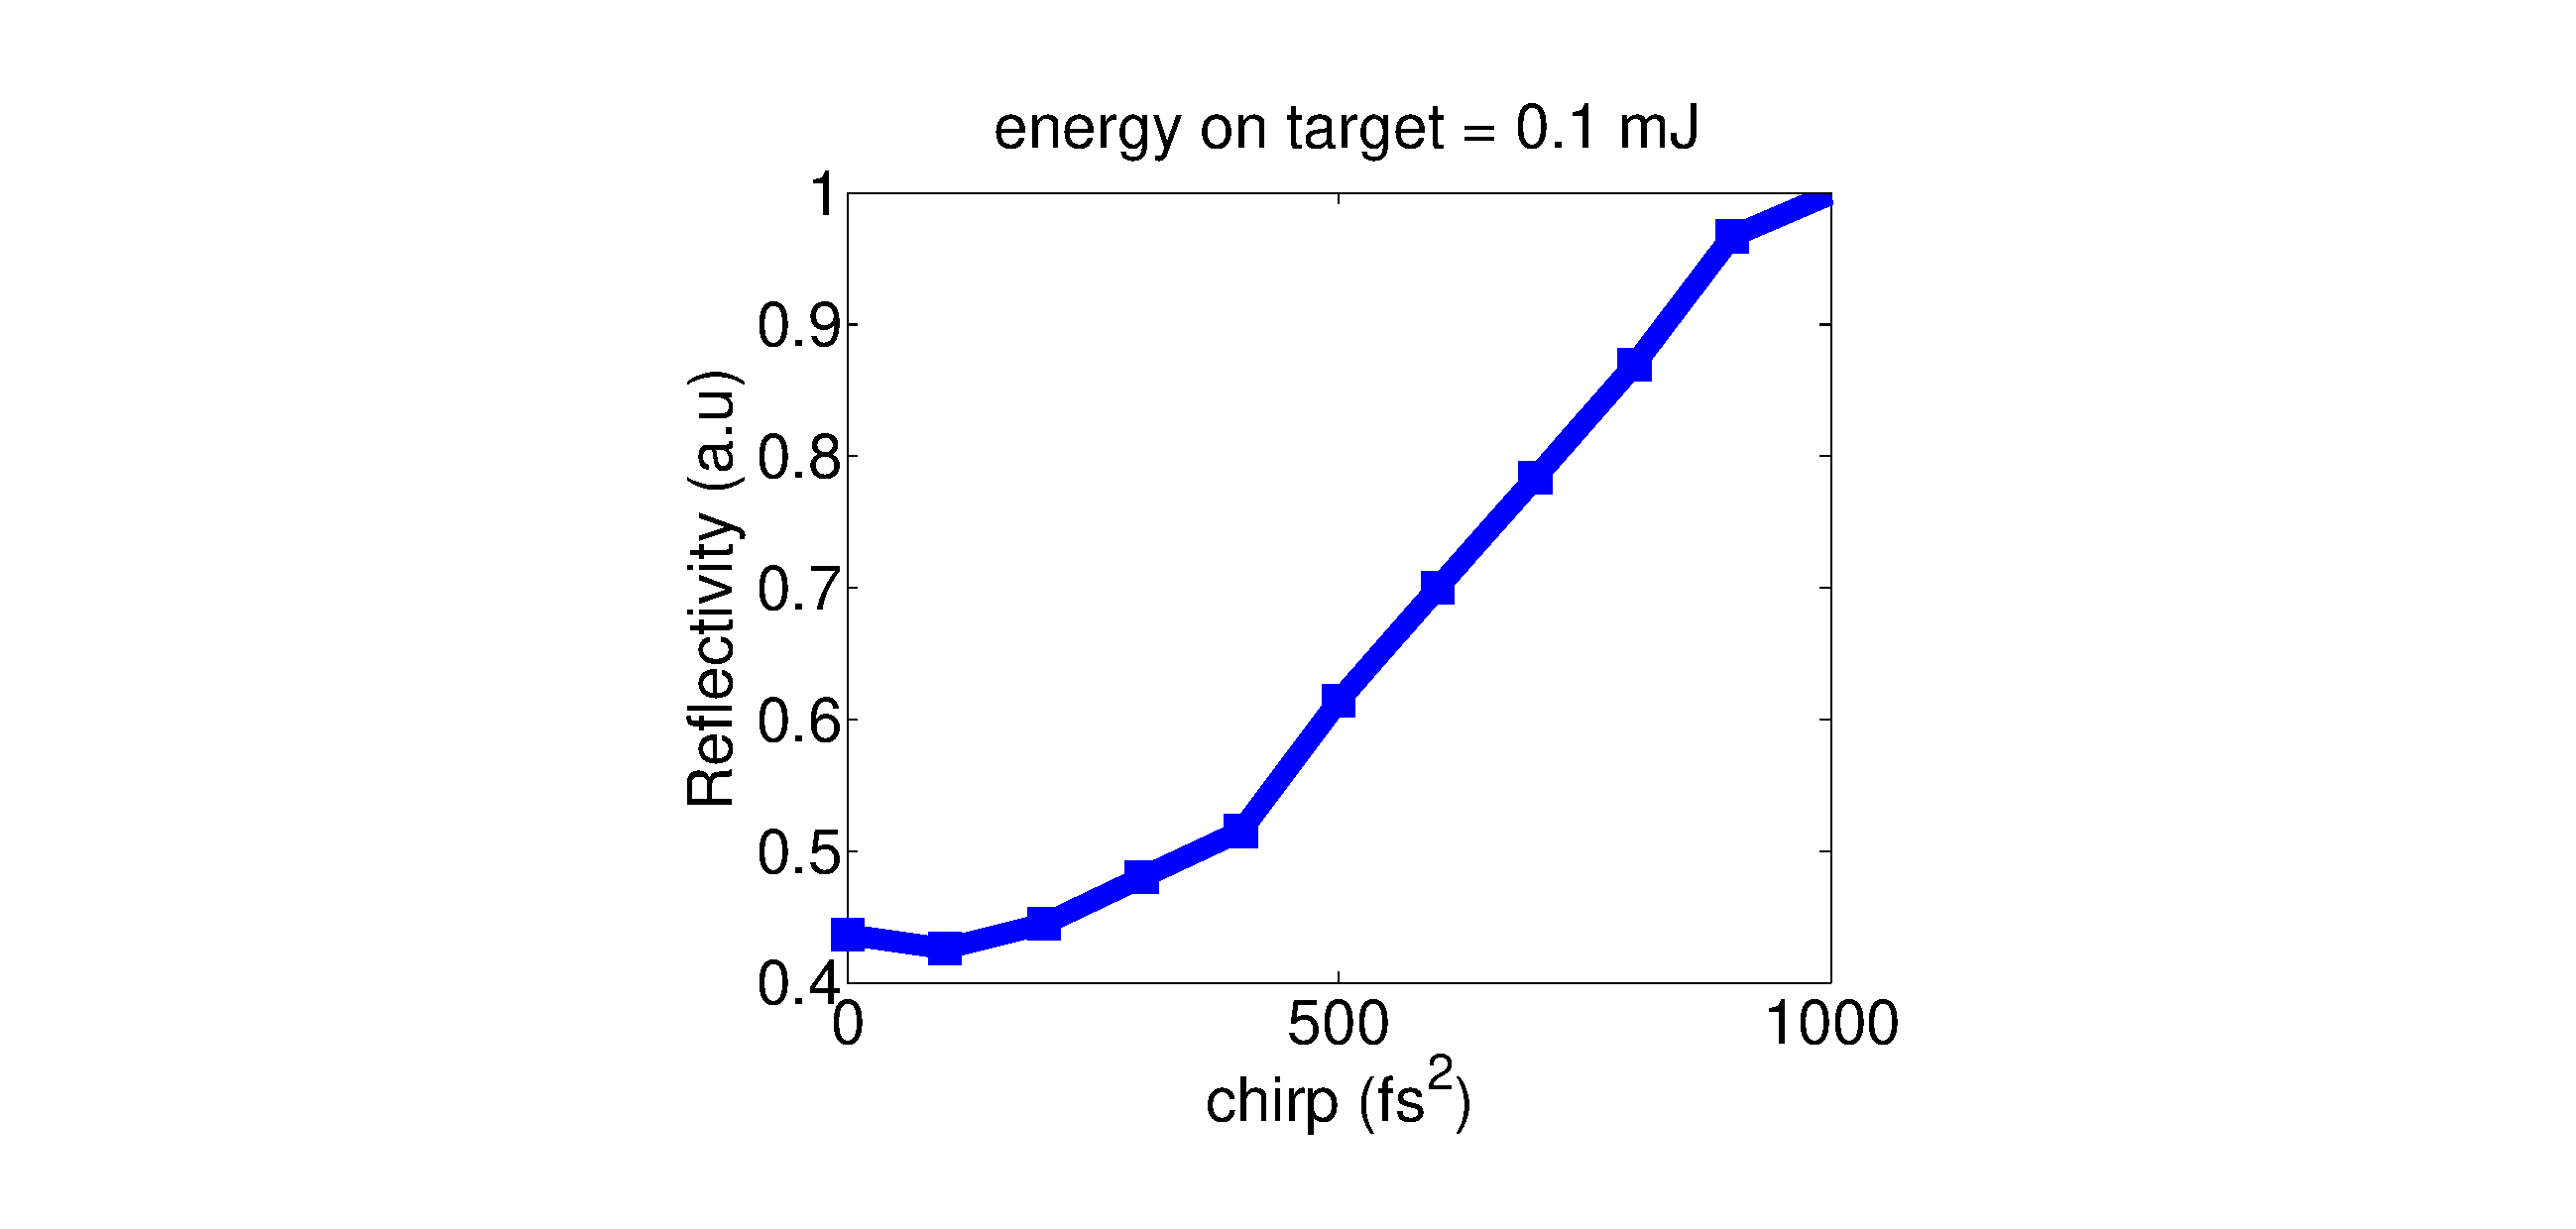
\includegraphics[width =\textwidth]{../chapitre7/images/Comparaisons-2.pdf}\\
\caption{\label{fig:Comparaisons} Evolution of the reflectivity as a function of chirp for an energy on target of $0.1$mJ. Each data point corresponds to the integration of 50 consecutive shots.}
\end{figure}

\noindent In order to investigate (ii), we measured the change in pulse reflectivity on target  in absence of prepulse. The pulse intensity on target is on the order of $\sim 10^{14}\,\mathrm{W/cm^2}$, and its temporal duration is $30\,\mathrm{fs}$.   Fig~\ref{fig:Comparaisons}(b) shows that a chirped pulse exhibits enhanced reflectivity. One possible explanation is that the plasma mirror is triggered sooner when the pulse is chirped. In conclusion, when a compressed prepulse is used to ionize a target prior to an interaction, spatio-temporal couplings (such as inhomogeneous compression) can lead to energy deposition not only dependent on the fluence . As a result, the plasma expansion can lead to high-order asymmetric plasma profiles.





\section{Perspectives for phase retrieval}\label{section:Phase retrieval perspective}

\subsection{Inversion problem}\label{subsection:Inversion problem}

Let's define what we call an "inversion problem". Suppose that we know the relation:
\begin{equation}
\label{eq:InversionEquation}
y = f(x)
\end{equation}
\noindent where $x$ is any unknown variable, and $y$ an "observable". An inversion problem simply consists in retrieving $x$ when $y$ is known.  For example, $y$ could be the fluence measured in 2 different planes along the propagation axis of a monochromatic laser beam. In this case, $f$ refers to Maxwell's equations and $x$, the fluence and phase in an arbitrary plane along the same axis of propagation. By measuring $y$, one could in principle retrieve $x$ using an available inversion algorithm like the Gerchberg-Saxton algorithm commonly employed for this particular problem \cite{hayes1983recursive,yang1994gerchberg}. One question naturally arises when one is faced with an inversion problem: is it really possible to invert the system. Or, to put in more mathematical terms: is $f$ injective ?\\

\noindent In our experiment, we measure the far-field intensity $I$ of the probe pulse, which according to Eq~\ref{eq:FarField2} takes the form:

\begin{equation}
\label{eq:InversionProblem} I= |\mathscr{F}( f )|^2
\end{equation}

\noindent where $f=\mathscr{F}[E_M] T$.\\

\noindent \g{We want to answer the following question:} is it possible to retrieve the complex transfer function $T$ from I ?

\subsection{One-dimension retrieval}

Without any further constraints, it is quite straightforward that a solution of Eq~\ref{eq:InversionProblem} is never unique because $f =\mathscr{F}^{-1}(I e^{i\phi})$ is always a solution, for any $\phi$ we consider. Therefore, the uniqueness can only arise from a constraint imposed on the function $f$. For example, a constraint used in optical retrieval~\cite{trebino2000frog,kane1993single,Kane2008}, where $f$ is a two-dimensional matrix, is that its rank is equal to one (ie the matrix is the product of a column times a line vector). If enough information is known about the object to be reconstructed from its Fourier modulus to ensure the uniqueness of the solution, a Fienup \cite{Fienup1987} inversion algorithm, which is described schematically in Fig~\ref{fig:DiagramRetrieval}, can be used. Every iteration, the reconstruction error $f$, calculated using $f'$ estimate, decreases.\\

\begin{figure}[H]
\centering
\includegraphics[width =0.9\textwidth]{../chapitre7/images/DiagramRetrieval.pdf}\\
\caption{\label{fig:DiagramRetrieval} Fienup phase retrieval principle}
\end{figure}


 
\noindent   In case of SDI, supposing the laser beam has a perfectly flat phase prior to focusing, the reference field $E_{ref}$ is obtained by a Fourier transform of the measured near-field square root intensity, or by an inverse Fourier transform of the square root intensity of the reflected field when $T = 1$.
When the plasma starts expanding or modifying the reflectivity over the $0^{th}$ order $E_{ref,\sigma}\equiv E_{ref,0}$, other diffracted orders which we generically label $E_{ref,\bar{\sigma}}$
remain unchanged as illustrated by Fig~\ref{fig:PrincipleSigmaConstraint}, which represents three spatially separated Gaussian sources, where only the central one is multiplied by an arbitrary transfer function $T$, represented in small insert at the top.

 \begin{figure}[H]
\centering
\includegraphics[width =0.7\textwidth]{../chapitre7/images/PrincipleSigmaConstraint.pdf}\\
\caption{\label{fig:PrincipleSigmaConstraint}Construction of object $f$: The central Gaussian source $E_{ref,\sigma}$ is multiplied by the plasma complex transfer function $T$ without affecting the other sources positioned symmetrically around $x=0$, which we define as $E_{ref,\bar{\sigma}}$}
\end{figure}

\noindent $E_{ref,\bar{\sigma}}$ will be the value of the field we impose in the Fienup-like retrieval algorithm represented in Fig~\ref{fig:DiagramRetrieval}. In Fig~\ref{fig:PhaseReconstruction1},we give an example of the results of the retrieval algorithm with three sources after 200 iterations for a complex function T, where $|T|=1$ and $\phi_T$ polynomial. The object $f$ is known on $\bar{\sigma}$, and we want to retrieve it on $\sigma$ only. In Fig~\ref{fig:PhaseReconstruction1}(a), we represent both its phase and superimpose the retrieved values after running the Fienup algorithm. In Fig~\ref{fig:PhaseReconstruction1}(b), we represent the Fourier transform modulus of the object and superimpose its retrieved modulus.\\

 \begin{figure}[H]
\centering
\includegraphics[width =\textwidth]{../chapitre7/images/PhaseReconstruction1.pdf}\\
\caption{\label{fig:PhaseReconstruction1} Phase reconstruction (a): initial modulus and phase of object on $\sigma$ (plain) and reconstructed object using Fienup algorithm (dotted). (b): constraint modulus in Fourier space (black plain) and resconstructed modulus (green dotted) after 200 iterations.}
\end{figure}

\noindent The retrieval error in Fourier domain is defined by the root mean square relation~\cite{Fienup1987}:
\begin{equation}
e = \biggl(\frac{\sum_{x}||F'(x)|-\sqrt{I(x)}|^2}{\sum_{x}I(x)}\biggr)^{1/2}
\end{equation}

\noindent where $F'$ is the retrieved Fourier transform and $\sqrt{I}$ its constraint (measured) modulus.

\noindent The retrieval error in the object domain on $\sigma$:
\begin{equation}
e = \biggl(\frac{\sum_{x\in \sigma}|f'(x)-f(x)|^2}{\sum_{x}|f'(x)|^2}\biggr)^{1/2}
\end{equation}


\noindent The employed algorithm is quite robust and always converges (final error in Fourier domain $e << 1$) for all the transfer functions T we imposed. However, the algorithm can converge in the Fourier domain without converging in the object domain.
Indeed, two very distinct objects can have the same Fourier transform modulus. In other words, the uniqueness of the inversion problem is not always ensured. This explains why the object error in Fig~\ref{fig:PhaseReconstruction1}(a) is much greater than the Fourier modulus error in Fig~\ref{fig:PhaseReconstruction1}(b). 

\noindent Phase retrieval has been an active and challenging field of research for over a century. So far, demonstrating the uniqueness of the solution for an arbitrary object support \footnote{Domain of definition of a function $f$ where $f \ne 0$} constraint is an open problem. Uniqueness has been demonstrated in restricted cases however:
 \begin{itemize} 
\item[$\bullet$]  For the one-dimensional inversion problem where both the support of f and $\mathscr{F}( f )$ are discrete, the uniqueness of the solution (supposing it exists, which is of course always the case experimentally) is ensured \cite{crimmins1983uniqueness} with the underlying hypothesis that two solutions $f_1$ and$f_2$ verify the relation $f_1 = a f_2(x + b)$ where $a,b \in \mathbb{R}$ are equivalent.
\item[$\bullet$]  The uniqueness of  phase for one and two-dimensional inversion problems for a real positive object has been demonstrated \cite{bruck1979ambiguity,hayes1982reconstruction}.
\item[$\bullet$] Holography principle: the object includes a delta function, also called reference point, sufficiently separated from the object to reconstruct \cite{fienup1983holographic,fienup1984experimental}. In this case phase reconstruction is possible.
\end{itemize}
\vspace{5px}

\noindent In our case, to address the problem of uniqueness, we run our retrieval algorithm on test functions where $|T| = 1$ and the phase of $T$ is taken of polynomial form:

\begin{equation}
P(x) = a_0 + a_1x + a_2 x^2+ .. a_6 x^6
\end{equation}

\noindent in the seven following cases: 
%\begin{tabular}{cc}
%&$(a_0,a_1,a_2,a_3,a_4,a_5,a_6) = $ & $(1,0,0,0,0,0,0)$\\
%& & ()
%\end{tabular}
\begin{equation} \label{eq1}
\begin{split}
(a_0,a_1,a_2,a_3,a_4,a_5,a_6) & = (1,0,0,0,0,0)\,\,\mathrm{(case 1)}\\
 & =(0,1,0,0,0,0)\,\,\mathrm{(case 2)}\\
  & =(0,0,1,0,0,0)\,\,\mathrm{(case 3)}\\
   & =(0,0,0,1,0,0)\,\,\mathrm{(case 4)}\\
    & =(0,0,0,0,1,0)\,\,\mathrm{(case 5)}\\
     & =(0,0,0,0,0,1)\,\,\mathrm{(case 6)}\\
      & =(1,1,1,1,1,1)\,\,\mathrm{(case 7)}\\
\end{split}
\end{equation}

\noindent with a maximum value of $\pi$. The corresponding result is given in Fig~\ref{fig:Symetric500iteration}. It appears that for cases 3 and 5, uniqueness is not ensured since the retrieved objects are different from the input object. We empirically found it was possible to drastically reduce these discrepancies by breaking the symmetry of the reference field on $\bar{\sigma}$ with respect to the origin as shown in ~\ref{subsection:Unicity solutions by break of symetry}. 

 \begin{figure}[H]
\centering
\includegraphics[width =\textwidth]{../chapitre7/images/Symetric500iteration.pdf}\\
\caption{\label{fig:Symetric500iteration}Amplitude and phase reconstructions}
\end{figure}

\newpage

\subsection{Modifying the reference probes to break the symmetry}\label{subsection:Unicity solutions by break of symetry}

So far, the reference field was constructed using 3 spatial Gaussian functions: one to which we apply the transfer function $T$ defined on $\sigma$, and 2 others, defined on $\bar{\sigma}$, symmetrically positioned with respect to the origin as already described in Fig~\ref{fig:PrincipleSigmaConstraint}. Here, we break this symmetry by positioning them at respectively $x= -30$ and $x=25$, instead of $x=\pm 25$. We then run the same retrieval algorithm on the previously defined 7 cases and find the results shown in Fig~\ref{fig:aSymetric500iteration} afer 200 iterations. The difference is striking: all cases converge to the right solutions in object domain as if uniqueness resulted from this break of symmetry. The residual errors in object domain is plotted in Fig~\ref{fig:errors}, where the symmetric and non symmetric case are compared: when the probes are not positioned symmetrically with respect to the object on $\sigma$, the final error is reduced by two orders of magnitude.

% These reference probe positions 
 \begin{figure}[H]
\begin{center}
\includegraphics[width =\textwidth]{../chapitre7/images/errors.pdf}\\
\caption{\label{fig:errors} Phase reconstruction error for a symmetric reference field on $\bar{\sigma}$ (blue) and when this symmetry is broken (red)}
\end{center}
\end{figure}


 \begin{figure}[H]
\centering
\includegraphics[width =\textwidth]{../chapitre7/images/aSymetric500iteration.pdf}\\
\caption{\label{fig:aSymetric500iteration} Amplitude and phase reconstructions for non symmetric reference field on~$\bar{\sigma}$}
\end{figure}

\newpage

\subsection{Two-dimensional retrieval ambiguities}

It is commonly stated that many phase retrieval problems can be solved in two dimensions when often they can't in one dimension. Such statement is the result of several successful empirical reconstructions in 2 dimensions \cite{fienup1987phase,fienup1984diffraction,napier1974inferring}. Since the late 70's, algebraic  approaches to the problem of phase inversion \cite{rosenblatt1984phase,barakat1984necessary} lead to the understanding of this singular two-dimensional behavior. The principle is simple: let's consider Eq~\ref{eq:trace1}, where $S$ is the expression of the discrete Fourier transform modulus of the function $f$ defined on a rectangle of size $N\times M$. One can define the polynomial in Eq~\ref{eq:trace2}, also known as the corresponding z-transform \cite{dudgeon1975existence}, where $z$ and $\eta $ are complex variables:



\begin{equation}
\label{eq:trace1}
S(k_x,k_y) = \frac{1}{NM}|\sum_{n}\sum_{m}f(x_n,y_m)\underbrace{e^{-i k_x ndx}}_{z=e^{-i k_x dx}}\underbrace{e^{-i k_y m dy }}_{\eta = e^{-i k_ydy }}|^2
\end{equation}

\begin{equation}
\label{eq:trace2}
P(z,\eta) = \frac{1}{NM}\sum_{n}\sum_{m}f(x_n,y_m)z^n \eta^m
\end{equation}

\noindent where $n$ and $m$ are integers corresponding to the index in the $x$ and $y$ directions respectively. Here, the inversion problem defined in  Eq~\ref{eq:trace1} is simply equivalent to the factorization of Eq~\ref{eq:trace2}. In other words, if by measuring $|P(z,\eta)|$ we can enumerate all its zeros\footnote{Roots of the polynomial. For polynomial P of degree N, if $z_{i\le i \le N}$ are the roots of P, then $P = \alpha \prod_{i} (z-z_i)$ where $\alpha \in \mathbb{C}$}, than $P$ and therefore $f$ is known. Many mathematical tools exist to deal with algebraic problems, and they allow to understand the singular difference between one and two-dimensional problems. Indeed, it has been shown~\cite{bruck1979ambiguity} that uniqueness emerges from the sufficient (but not necessary) condition that the factorization of Eq~\ref{eq:trace2} is not possible. On the one hand, it is always possible in 1D to factorize a polynomial. One understands that in that case, the uniqueness of the inversion problem requires a strong support constraint. On the other hand, the probability of finding non-factorisable solutions increases in 2D~\cite{bose1982applied,tzafestas1986state} which explains why, in general, 2D retrieval algorithms are more robust. \\

\noindent This being said, we ran the SDI reconstruction algorithm presented in section~\ref{subsection:Inversion problem} using simulated 2D traces and found that the reconstruction performance was slightly, but not significantly, increased for the pathological cases presented in \ref{subsection:Inversion problem} (where the probe is symmetric with respect to the object to reconstruct). However, the counterpart is a quadratic increase in computing time. When the probe is asymmetric, the reconstruction is very good and converges in less iterations, as illustrated with the example given in Fig~\ref{fig:2D_reconstruct}. Here, we present the phase object (left) and its 2D reconstruction after 20 iterations (right).

 \begin{figure}[H]
\centering
\includegraphics[width =\textwidth]{../chapitre7/images/2D_reconstruct.pdf}\\
\caption{\label{fig:2D_reconstruct} Result of central object phase reconstruction after 20 iterations using non symmetrically distributed sources. The residual reconstruction error measured in the Fourier modulus is $e = 5\times 10^{-4}$}
\end{figure}





\section{Conclusion and perspectives}

We have seen how inserting a simple periodic transmission mask in the path of the intense IR probe, we can use the higher order diffraction spot at the focus on target as a reference for a SDI measurement. When plasma expansion is induced by the delayed prepulse, the change in reflectivity and phase of the probe can in principle be fully retrieved using an inversion algorithm. In our experiment, the image quality was no sufficient (limited dynamic range of CCD, diffuser grain size, low signal to noise ratio due to background radiation) to implement such an algorithm. Moreover, we realized after the experiment that breaking the central symmetry in the focusing plane would be an excellent way to increase the retrieval accuracy. One easy solution to do this is to reflect one of the first-order diffraction spots on the plasma rather than on the $0^{th}$ order. 
This will be tested in future experiments in order to fully reconstruct the 2D plasma expansion profile from its instant of creation.
























